\section{Evaluación de Desempeño y Tiempos de Ejecución}

Para validar las hipótesis de complejidad asintótica planteadas, se realizaron pruebas de estrés comparando las tres versiones del algoritmo.

\subsection{Tabla Comparativa de Rendimiento}
La siguiente tabla muestra el tiempo de respuesta (en segundos) para distintos rangos de búsqueda ($MAX$). Se observa cómo el algoritmo original se vuelve inviable rápidamente, mientras que las versiones de criba mantienen tiempos de respuesta casi instantáneos.

\begin{table}[H]
\centering
\resizebox{\textwidth}{!}{
    \begin{tabular}{|l|c|c|c|}
    \hline
    \textbf{Rango (MAX)} & \textbf{Algoritmo Original ($O(n^2)$)} & \textbf{Criba Nativa ($O(n \log n)$)} & \textbf{Criba NumPy ($O(n \log n)$)} \\ \hline
    10.000               & 3.18s                                  & 0.008s                                & 0.013s                               \\ \hline
    50.000               & 84.2s                                  & 0.029s                                & 0.049s                               \\ \hline
    100.000              & 370s                                   & 0.068s                                & 0.072s                               \\ \hline
    150.000              & 837s                          & \textbf{0.108s}                                & \textbf{0.104s}                      \\ \hline
    200.000              & Inviable                               & 0.155s                                & 0.130s                               \\ \hline
    250.000              & Inviable                               & 0.207s                                & 0.172s                               \\ \hline
    500.000              & Inviable                               & 0.508s                                & 0.332s                               \\ \hline
    1.000.000            & Inviable                               & 1.416                                 & 0.637s                               \\ \hline
    \textbf{2.000.000}   & Inviable                      & \textbf{3.608}                                 & \textbf{1.320s}                      \\ \hline
    \end{tabular}
    }
\caption{Comparativa de tiempos de ejecución en segundos.}
\end{table}

Como se observa en los resultados resaltados para $\text{MAX} = 100.000$, la versión nativa de Python (0.068s) logra ser ligeramente más rápida que la versión optimizada con NumPy (0.072s).
Este comportamiento, aunque contraintuitivo a primera vista, se debe al costo de inicialización u overhead de la librería NumPy. Al trabajar con rangos ``medianos'', el tiempo que NumPy dedica a reservar memoria contigua y convertir los tipos de datos de Python a C es superior al tiempo que ahorra mediante la vectorización. La versión nativa, al no tener este costo de arranque, resulta más eficiente en este escenario. \\

Sin embargo, el punto de inflexión se manifiesta claramente a partir de $\text{MAX} = 150.000$, donde la versión con NumPy ($0.104$s) comienza a superar a la nativa ($0.108$s). A medida que el rango se extiende, la eficiencia de las operaciones vectorizadas compensa con creces los costos iniciales de configuración de la librería. Esta tendencia se consolida en el escenario de $\text{MAX} = 2.000.000$, donde NumPy logra procesar el conjunto de datos en aproximadamente un tercio del tiempo requerido por la implementación nativa ($1.320$s frente a $3.608$s), demostrando
una mayor escalabilidad para procesar grandes volúmenes de información.

\subsection{Representación Gráfica de los Resultados}
A continuación, se presentan los gráficos obtenidos a partir de las mediciones de tiempo. Estas visualizaciones permiten contrastar el comportamiento de las tres implementaciones y observar cómo la teoría de la complejidad asintótica se traduce en tiempos de ejecución reales sobre el hardware de prueba. \\

Las gráficas se dividen en tres enfoques:
\begin{itemize}
    \item \textbf{Escala General:} Comparación del impacto drástico entre el algoritmo original ($O(n^2)$) y la criba optimizada, donde se evidencia la inviabilidad del primero para rangos extensos.
    \item \textbf{Análisis de Eficiencia Relativa:} Un acercamiento a la competencia entre la versión nativa y la de NumPy para identificar el umbral donde la vectorización comienza a ser superior.
    \item \textbf{Escalabilidad Log-lineal:} El comportamiento de la solución definitiva en rangos de hasta dos millones de números, verificando la estabilidad del crecimiento $O(n \log n)$.
\end{itemize}

\begin{figure}[H]
    \centering
    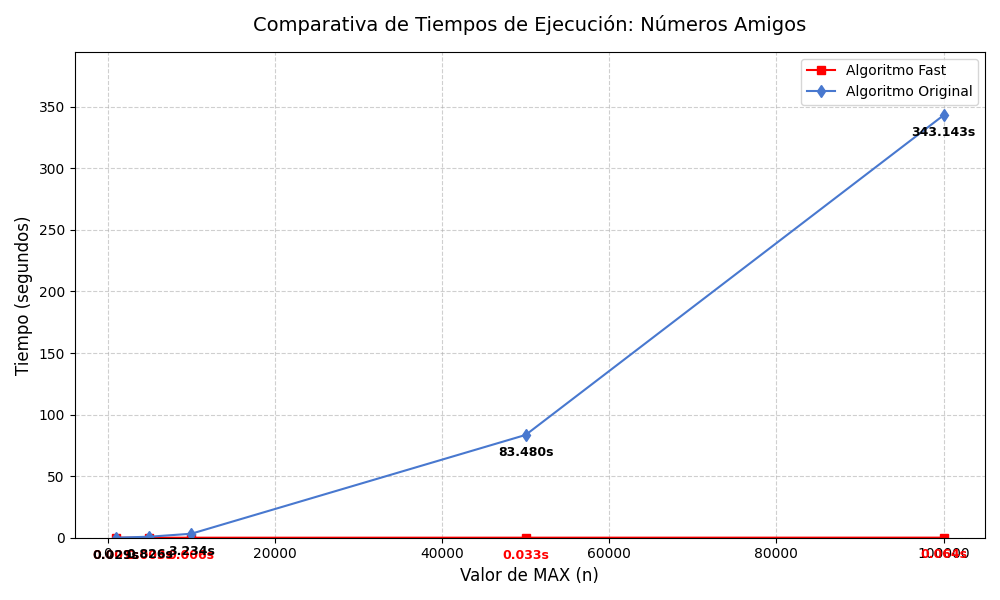
\includegraphics[width=1.0\textwidth]{../../Graficos/comparacion.png}
    \caption{Comparativa de tiempos de ejecución entre el algoritmo original $O(n^2)$ y el algoritmo optimizado ("Fast"). Se observa el crecimiento exponencial del modelo ineficiente frente a la escala casi plana de la criba optimizada.}
    \label{fig:comparacion_drastica}
\end{figure}

\begin{figure}[H]
    \centering
    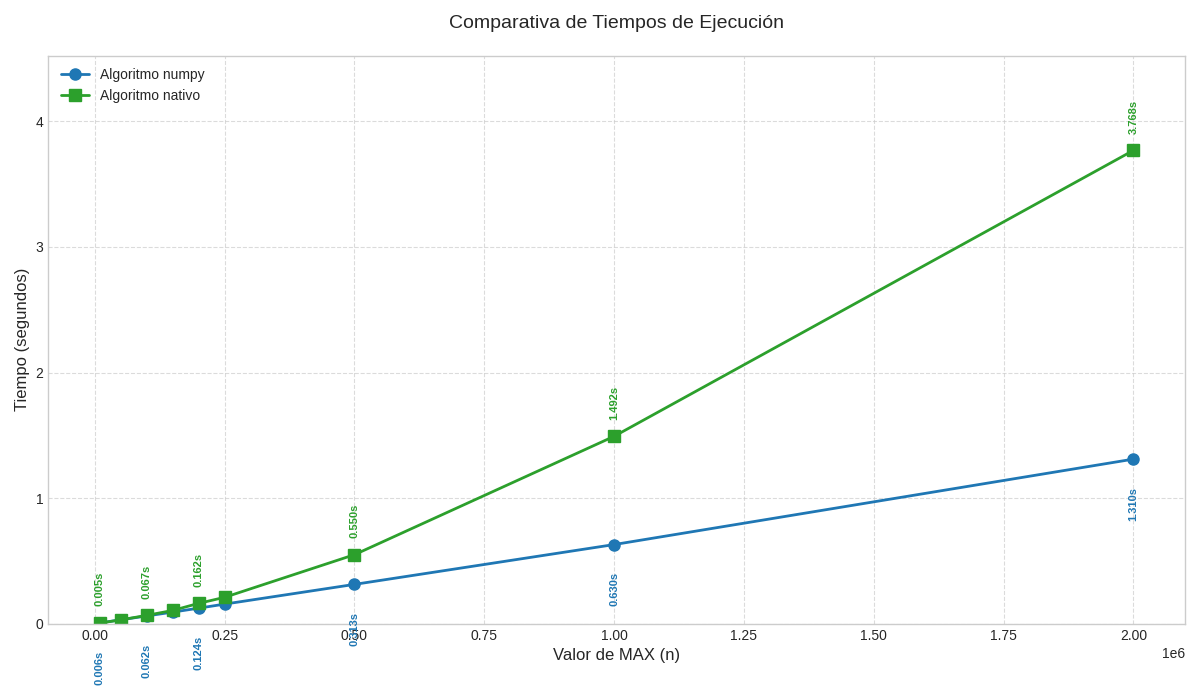
\includegraphics[width=1.0\textwidth]{../../Graficos/nativo_vs_numpy.png}
    \caption{Comparativa detallada entre la Criba Nativa (en verde) y la Criba con NumPy (en azul). Se observa el overhead inicial de NumPy para rangos bajos y el punto de inflexión donde la vectorización comienza a ofrecer un mejor rendimiento.}
    \label{fig:comparacion_cribas}
\end{figure}

\begin{figure}[H]
    \centering
    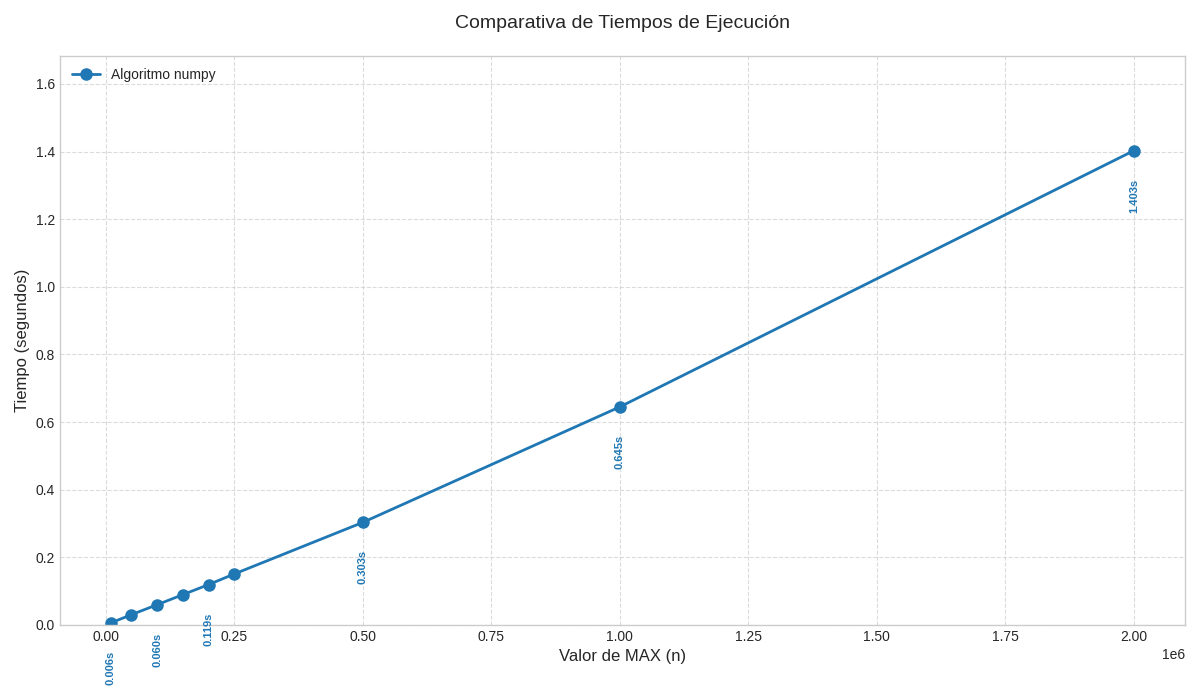
\includegraphics[width=0.85\textwidth]{../../Graficos/grafico_algoritmo_optimizado.png} 
    \caption{Tiempos de ejecución del algoritmo optimizado con NumPy. Se observa una tendencia de crecimiento log-lineal ($O(n \log n)$), permitiendo procesar un rango de 2.000.000 de números en apenas segundos.}
    \label{fig:grafico_numpy}
\end{figure}
